\section{Virtueller Speicher}
Prozesse bekommen vom OS Speicher zugeteilt und das OS schaut, dass sich die Prozesse nicht gegenseitig stören.\\
\textcolor{myblue}{Lösung}: Die Prozesse kennen nur virtuelle Adressen. Das MMU übersetzt virtuelle Adresse in physische Adresse. Das OS konfiguriert einen MMU pro Prozess. \\
\textcolor{myblue}{MMU}: Memory Management Unit übersetzt virtuelle in physische Adresse.\\
\textcolor{myblue}{Page}: Virtueller Adressraum besteht aus Pages, eine Page hat jedoch keinen physischen Speicher. Sie benötigt einen Speicherort (Hauptspeicher/Sekundärspeicher).\\
\textcolor{myblue}{Frames}: Hauptspeicher wird in Frames aufgeteilt, in ein Frame passt genau eine Page. Ein Frame = eine Page.\\
\textcolor{myblue}{Virtueller Adressraum/Pagetable}: Pro Prozess ein virtueller Adressraum. \\
- Pro Prozess gibt es eine Pagetable (Mapping Tabelle)\\
- OS verwaltet, welche Pages wann wo liegen müssen. MMU kennt nur den
Hauptspeicher dh. MMU kann nur sagen ob Page, resp. zu Page
gehörendes Frame im Hauptspeicher ist.\\
\textcolor{myblue}{Status-Bit Used (P-Bit)}: Zeigt, ob Page used =1 oder unused = 0 ist.\\
\textcolor{myblue}{Interprozesskommunikation (IPC)}: \textbf{Shared Memory}: Prozesse teilen sich den
Speicher -> kein Schutz. \textbf{Message Passing}: OS kopiert Daten, sicher aber auch Overhead.\\
\textcolor{myblue}{Paging}: Verwaltung von pageorientiertem Speicher (Laden von Pages
etc.)\\
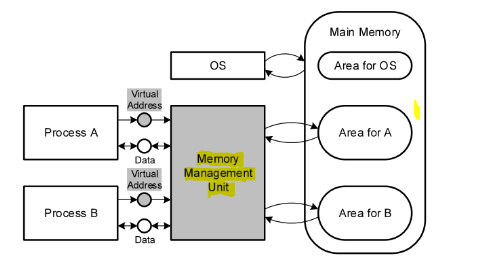
\includegraphics[width=\columnwidth]{mmu}
\subsection{Single-Level Page Table}
Für jede mögliche Page einen Eintrag. Die Grösse hängt vom virtuellen Adressraum ab. Lookup sehr schnell aber kann sehr schnell sehr gross werden.\\
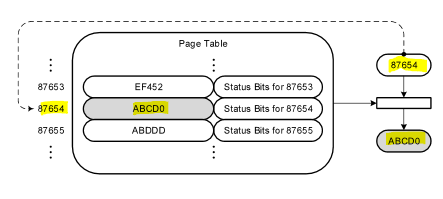
\includegraphics[width=\columnwidth]{single_level_page_table.png}
\subsection{Two-Level Page Table}
Page Number wird in Directory Index \& Page Table Index aufgeteilt\\
\vspace{-0.2cm}
\begin{enumerate}
	\item Page Table in Directory finden
	\vspace{-0.2cm}
	\item Table Index in Page Table finden
\end{enumerate}
\vspace{-0.2cm}
Viele Page Tables, Page Directory zeigt auf Page Tables\\
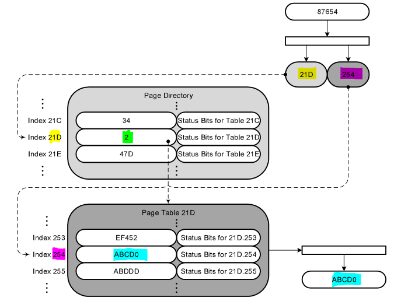
\includegraphics[width=\columnwidth]{two_level_page_table.png}
\subsection{Speicherfreigabe}
\textcolor{myblue}{Explizit}: Programmierer bestimmt, wann Speicher freigegeben wird.
Nur im OS ist explizite Speicherverwaltung möglich. →Mögliche Speicherlacks,
falls nicht verwendeter Speicher nicht mehr freigegeben wird.
\textcolor{myblue}{Implizit}: Speicher wird automatisch freigegeben, wenn er nicht benötigt wird.
Dies geschieht in der App (JVM, Python, ...)
\subsection{Befehle}
\textcolor{myblue}{Malloc(s)}: Alloziiert Speicherblock mit Grösse S.\\
\textcolor{myblue}{Free(*p)}: Gibt einen Speicherblock frei, der an Adresse p beginnt.\\
Malloc und free gehören wie Klammerpaare zusammen, damit es keine Speicherlacks gibt.
\textcolor{myblue}{Interne Fragmentierung}: Heap reserviert einen grösseren Speicherblock, als
angefragt wurde. Der überschüssige Speicher wird nicht verwendet.\\
\textcolor{myblue}{Externe Fragmentierung}: Das Programm reserviert immer wieder Speicher und
gibt ihn unregelmässig wieder frei. Über Längere Zeit entstehen kleine Löcher,
die aber, trotz in der Summe genügend gross wären, nicht in der Lage sind
grösseren Speicher zu reservieren.\\
\subsection{Suchalgorithmen}
\textcolor{myblue}{First fit}: Erste passende Lücke\\
\textcolor{myblue}{Next fit}: Erste passende Lücke nach zuletzt verwendetem Bereich\\
\textcolor{myblue}{Best fit}: Durchsucht alle Lücken nach der passendsten.\\
\textcolor{myblue}{Worst fit}: Durchsucht alle Lücken nach der Grössten\\
\textcolor{myblue}{Quick fit}: Erstes Element mit kleinster passenden Grösse\\
\textbf{Nachteil}: Nachbarn schwer zu finden.\\
\subsection{Paging}
\textcolor{myblue}{Dirty Bit}: Page im Hauptspeicher ist anders als im sekundären Speicher.\\
\textcolor{myblue}{Accessed Bit}: Page wurde kürzlich von Prozess verwendet → wird von MMU
gesetzt.\\
\textcolor{myblue}{Page Fault}: Wird gesetzt, wenn die referenzierte Page nicht im Hauptspeicher
ist.\\
\textcolor{myblue}{Bsp}\\
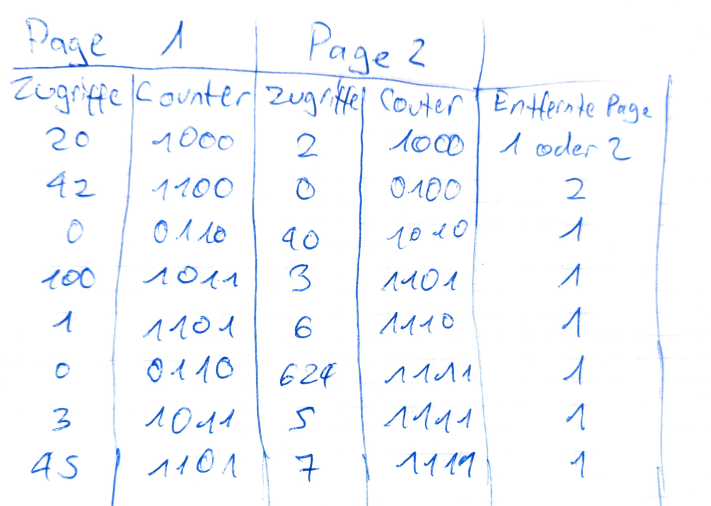
\includegraphics[width=\columnwidth]{nfu_with_aging.png}
\textcolor{myblue}{Working Set}: Wenn Alter >= Limit, dann wird Page entfernt, sonst bleibt sie.\\
Bsp. Limit des Alters zusätzlich 10\\
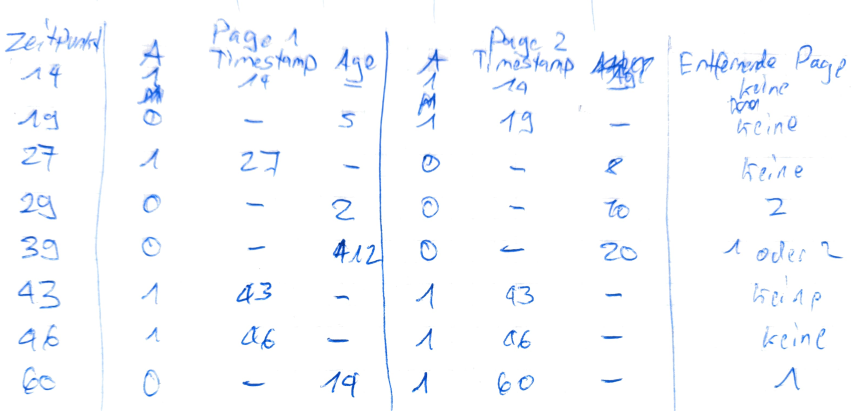
\includegraphics[width=\columnwidth]{working_set.png}